\section{Implementation}
\label{sec:implementation}

\subsection{Modulation}
\subsubsection{Triangle Wave Generator}
The topology implemented for this subcircuit was found in \citetitle{TriangleWaveTopology}\cite{TriangleWaveTopology}. 
It uses an integrator to generate a ramp from the output of a non-inverting schmitt trigger. 
This ramp is fed into the input of the schmitt trigger. When the ramp reaches a schmitt trigger threshold, the polarity of the schmitt trigger output reverses, forcing the integrator to ramp in the opposite direction. 
High precision, rail-to-rail opamps and E96 resistors ensure the amplitude and offset tolerances were met. 

Figure \ref{fig:triangleWaveGeneratorSchematic} shows the schematic, and Figure \ref{fig:triangleWaveGeneratorTestBench} shows the testbench used to test it. 
The Spice error log shows the results of the measurement directives.
The offset is 0.003V and the peak-to-peak voltage is 2.001 V.
The steady-state frequency is measured as 11.3532 Hz.
Each of these falls within the tolerances presented in Section \ref{sec:specificationTriangleWaveGenerator}.
A cutting of the waveform produced can be found in Figure \ref{fig:triangleWaveGeneratorWaveform}. 


\begin{figure}[H]
    \centering 
    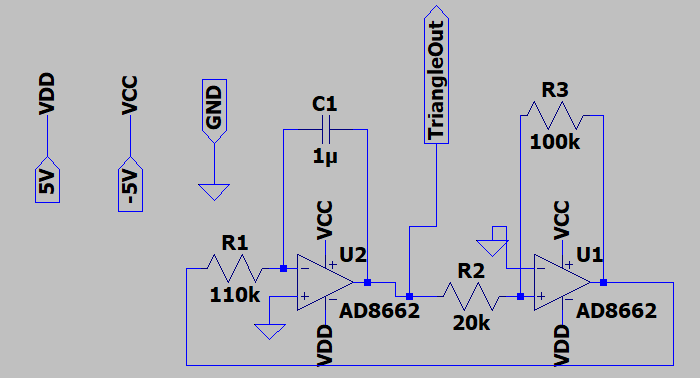
\includegraphics[width=\textwidth]{../Circuits/Images/TriangleWaveGenerator/schematic}
    \caption{A screencap of the Triangle Wave Generator Subcircuit}
    \label{fig:triangleWaveGeneratorSchematic}
\end{figure}

\begin{figure}[H]
    \centering 
    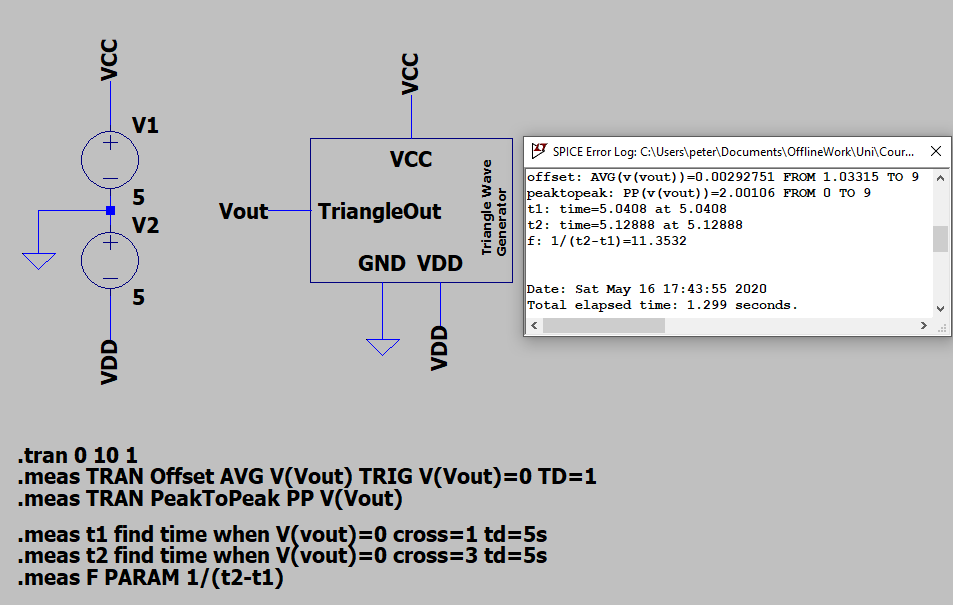
\includegraphics[width=\textwidth]{../Circuits/Images/TriangleWaveGenerator/TestBenchScreencap}
    \caption{A screencap of the Triangle Wave Generator Subcircuit}
    \label{fig:triangleWaveGeneratorTestBench}
\end{figure}

\begin{figure}[H]
    \centering 
    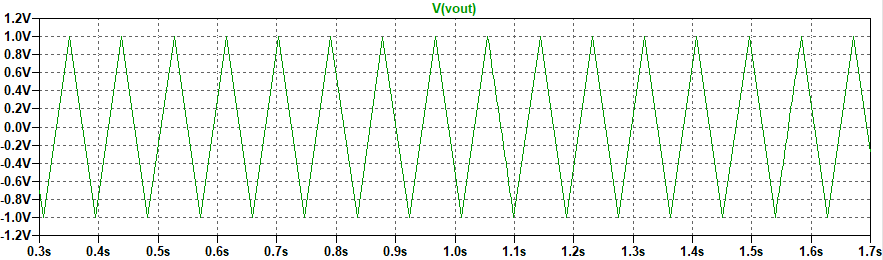
\includegraphics[width=\textwidth]{../Circuits/Images/TriangleWaveGenerator/OutputWaveform}
    \caption{A screencap of the Triangle Wave Generator Subcircuit}
    \label{fig:triangleWaveGeneratorWaveform}
\end{figure}

\subsubsection{VCO}
The VCO subcircuit is based on the LTC6990 VCO IC. 
$K_{VCO}$ and the centre frequency are set using E96 resistors.
The LTSpice schematic was adapted from a circuit generatd automatically on an online design tool provided by Analog Devices\footnote{\url{http://beta-tools.analog.com/timerblox/LTC6990}}.
The schematic is shown in Figure \ref{fig:VCOSchematic}.

The testbench varies the control voltage VC and takes frequency measurements at the appropriate times. 
The testbench is shown in Figure \ref{fig:VCOTestBench}.
The waveform produced is shown in Figure \ref{fig:VCOTestBenchWaveform}.

The measurements showed that the centre` frequency ($F_{Centre}$) is 39842 Hz and the Bandwidth of the FM Modulated signal is 7905.5 Hz.
This falls within the tolerances presented in Section \ref{sec:specificationVCO}.

This IC shifts the phase of the signal by $\pi$ radians, the FM signal frequency increases when VC drops and vica versa. 
The VCO will need to account for this. 

\begin{figure}[H]
    \centering 
    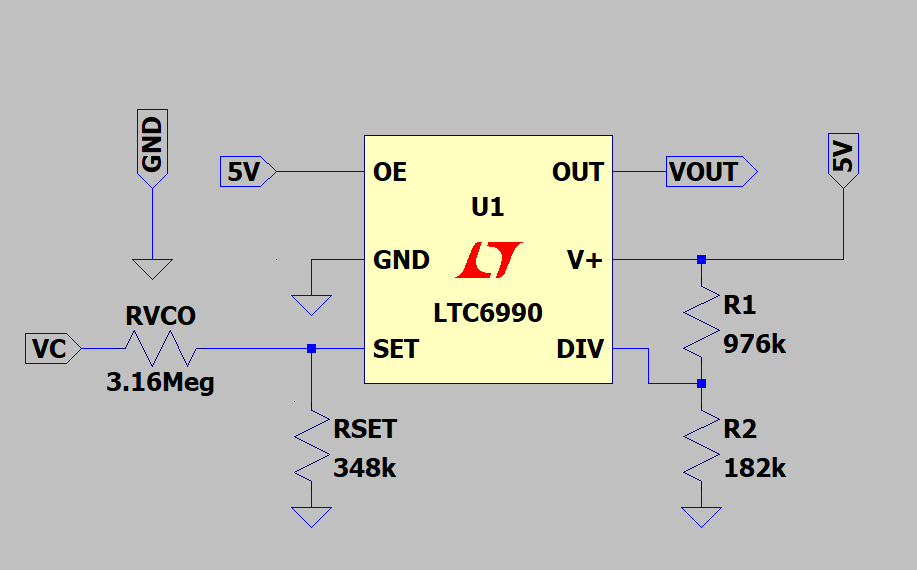
\includegraphics[width=\textwidth]{../Circuits/Images/VCO/Schematic}
    \caption{A screencap of the VCO Subcircuit}
    \label{fig:VCOSchematic}
\end{figure}

\begin{figure}[H]
    \centering 
    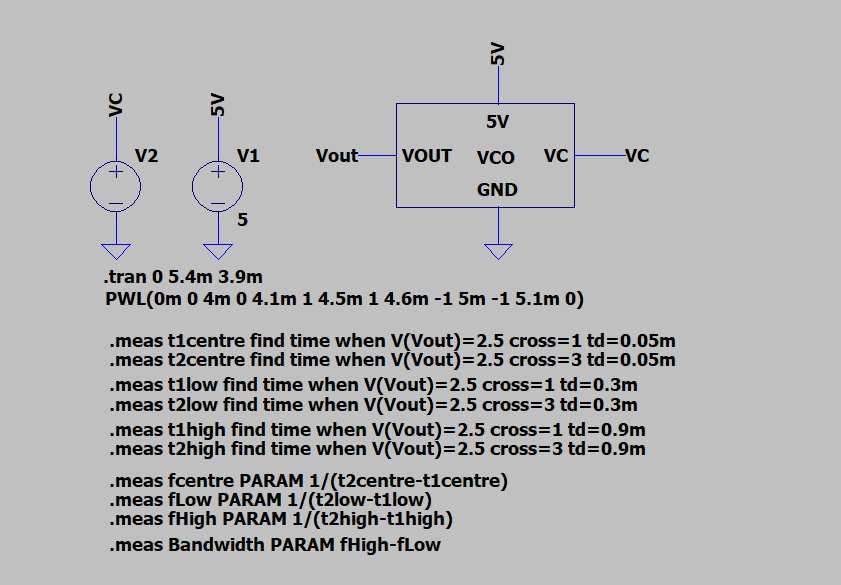
\includegraphics[width=\textwidth]{../Circuits/Images/VCO/TestBenchScreencap}
    \caption{The testbench fort the VCO Subcircuit}
    \label{fig:VCOTestBench}
\end{figure}

\begin{figure}[H]
    \centering 
    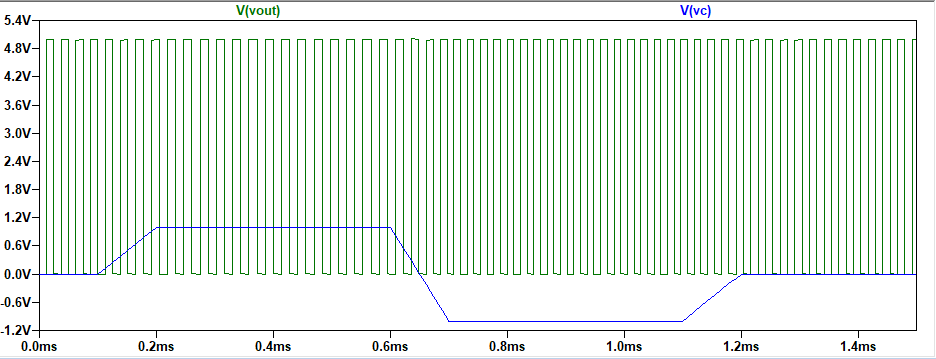
\includegraphics[width=\textwidth]{../Circuits/Images/VCO/TestBenchWaveform}
    \caption{The Waveform produced by the VCO Testbench}
    \label{fig:VCOTestBenchWaveform}
\end{figure}

\subsubsection{Transmission Amplifier}
Due to the low power requirements of the MOSFET, a SOT-23 package was chosen to conserve space and money. 
The Infineon IRLML6344\footnote{\url{https://uk.rs-online.com/web/p/mosfets/9134070/}} was used in the simulated version shown in Figure \ref{fig:TransmissionAmpSchematic} as it meets the power requirements discussed in Section \ref{sec:specificationTransmissionAmplifier} but any SOT-23 device could be used.

The testbench contains an Butterworth-Van Dyke equivalent circuit of a Piezo with parameters taken from experimental data presented by \citeauthor{equivalentCircuit} in their \citeyear{equivalentCircuit} paper\cite{equivalentCircuit}.

Figure \ref{fig:TransmissionAmpTestBenchWaveform} shows the mock VCO output super imposed over the current through the resistor R1.
It shows the constant charge and discharge of the capacitor C1, demonstrating that the MOSFET is able to induce mechanical oscillation on this mock transducer.

\begin{figure}[H]
    \centering 
    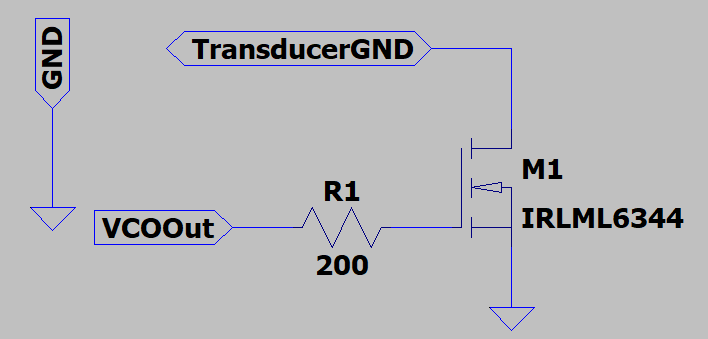
\includegraphics[width=\textwidth]{../Circuits/Images/TransmissionAmp/Schematic}
    \caption{A screencap of the VCO Subcircuit}
    \label{fig:TransmissionAmpSchematic}
\end{figure}

\begin{figure}[H]
    \centering 
    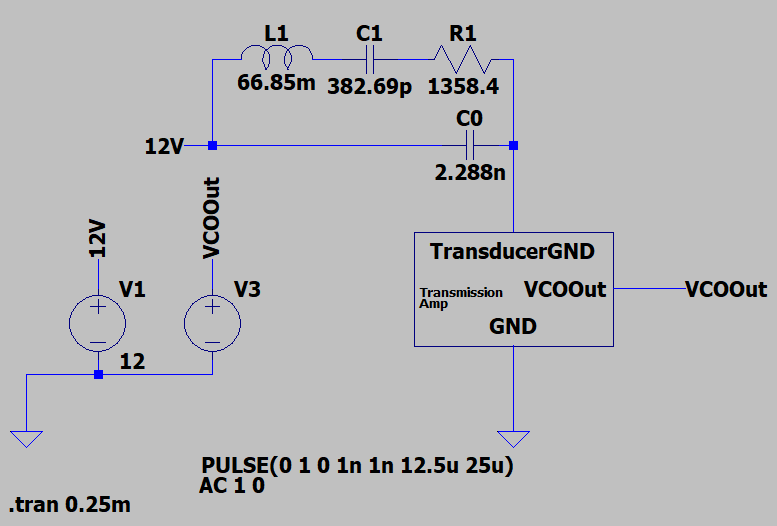
\includegraphics[width=\textwidth]{../Circuits/Images/TransmissionAmp/TestBenchScreencap}
    \caption{The testbench fort the VCO Subcircuit}
    \label{fig:TransmissionAmpTestBench}
\end{figure}

\begin{figure}[H]
    \centering 
    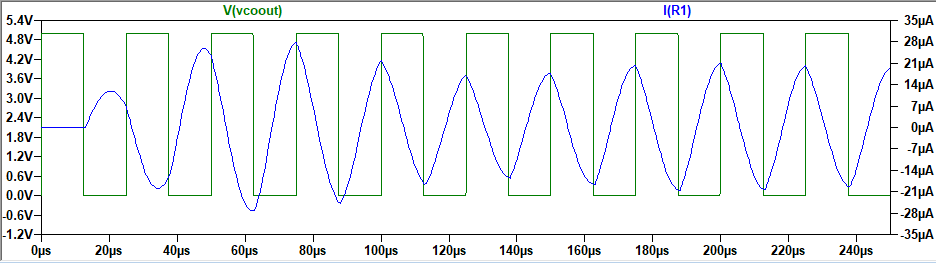
\includegraphics[width=\textwidth]{../Circuits/Images/TransmissionAmp/TestBenchWaveform}
    \caption{The Waveform produced by the VCO Testbench}
    \label{fig:TransmissionAmpTestBenchWaveform}
\end{figure}

\subsection{Demodulation}

\subsubsection{Pre-Amp}
The pre-amp was implemented using a non-inverting op-amp amplifier. 
This was to make setting the gain simple and to minimise costs. 
A high-speed op-amp chosen to reproduce any of the square wave characteristics that were transmitted by the modulation stage.

Figure \ref{fig:preAmpSchematic} shows the schematic for the preamp.
The parameters for the resistances are set by the testbench.

Figure \ref{fig:preAmpTestBench} shows the test bench. 
The gain is stepped across the range given in Section \ref{sec:specificationPreAmp}.
Parameters passed to the pre-amp block for R1 and R2 are calculated \(R1 = Rbase = 1k\) and \(R2 = Rbase \times gain\).
The input amplitude is reduced by the same factor that the gain is increased to approximate the gain of the system increasing to compensate for greater attenuation.
At each step the 3db point is calculated to give an approximation of the system bandwidth from 0 - 3db point. 
Figure \ref{fig:preAmpTestBenchOutput} shows the output of the measure directive, showing that the bandwidth requirements given in Section \ref{sec:specificationPreAmp} have been met.  

\begin{figure}[H]
    \centering 
    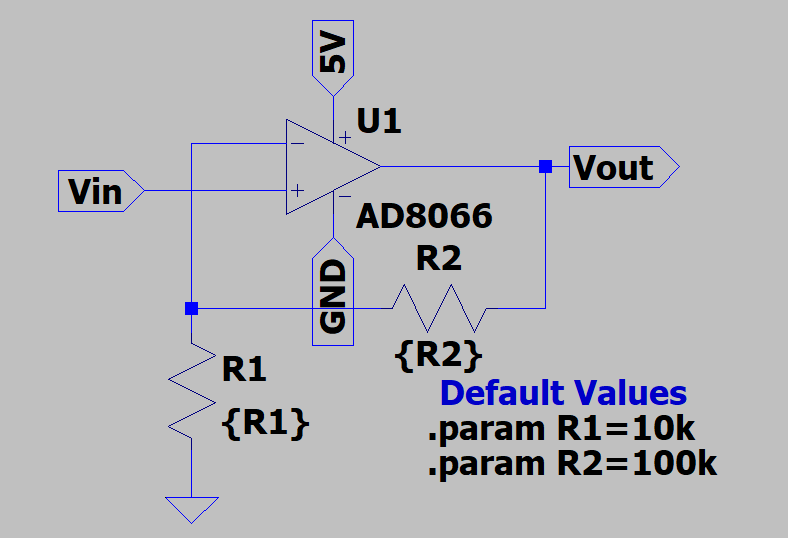
\includegraphics[width=\textwidth]{../Circuits/Images/Pre-Amp/Schematic}
    \caption{A screencap of the VCO Subcircuit}
    \label{fig:preAmpSchematic}
\end{figure}

\begin{figure}[H]
    \centering 
    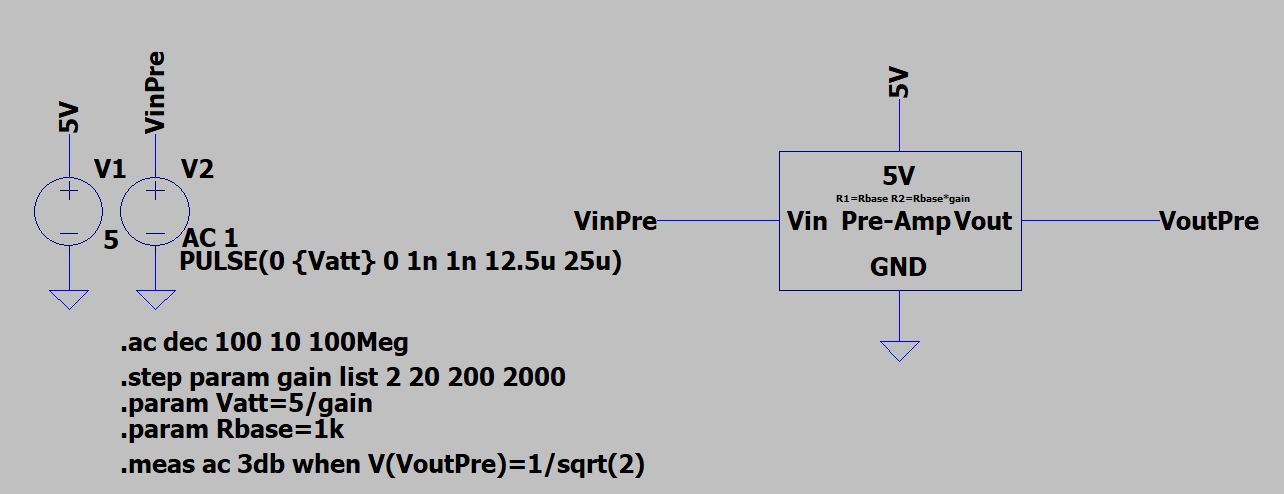
\includegraphics[width=\textwidth]{../Circuits/Images/Pre-Amp/TestBenchScreencap}
    \caption{The testbench fort the VCO Subcircuit}
    \label{fig:preAmpTestBench}
\end{figure}

\begin{figure}[H]
    \centering 
    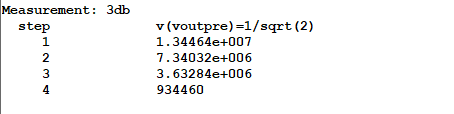
\includegraphics[width=\textwidth]{../Circuits/Images/Pre-Amp/TestBenchOutput}
    \caption{The Waveform produced by the VCO Testbench}
    \label{fig:preAmpTestBenchOutput}
\end{figure}

